\chapter{Generalized additive mixed models with kernel smoothers}
	
	\section{Introduction}
	\label{s:intro}
	% the problem of interest
	Geographically heterogeneous disease rates are of common interest in epidemiology studies since local high or low rates may serve as a surrogate for space-related risk factors such as environmental exposures and local healthcare access or quality. While traditional geographic modeling methods focus on analyzing aggregated area-level data that treat area-defined partitions as one unit, more recent spatial epidemiology studies avoid aggregation bias and the ecological fallacy by modeling individual-level data that may be collected longitudinally over time.  With accurate records of geospatial information (frequently longitude and latitude), researchers generally assume an underlying smooth surface for modeling the heterogeneity of disease risk over a given geospatial region, regardless of borders of inner areas. Based on this assumption, the estimation of the surface is an essential component in spatial data analysis. 
	
	Due to the complex nature of geospatial disease risk, it is not feasible to assume a parametric form to model the underlying risk surface in most cases. As such, nonparametric methods are popular in spatial effects modeling. Under a frequentist estimation framework, popular nonparametric methods include kernel and spline smoothers. Kernel smoothers utilize locally weighted models while spline smoothers are defined by a basis expansion of the design matrix over the full predictor support. In this work we consider locally weighted regression (LOESS) as proposed by \citet{cleveland1979robust}. LOESS assumes local (weighted) polynomial relationship between response and explanatory variables and was applied to geospatial analysis by \citet{brunsdon1996geographically} among others. One advantage of LOESS for spatial analyses is that it intuitively adapts to changing population densities by varying the size of the smoothing neighborhood based on the local data density given a fixed span size (typically defined as the proportion of observations used for local regressions). %One popular way to choose an optimal span size is to use Akaike information criterion (AIC). \citep{akaike1998information}
	
	In addition to spatial risk pattern estimation, confounding variables, such as biomarkers in studies on public health, should be included in spatial models. Generalized additive models (GAMs) \citep{hastie1990generalized} offer a framework for incorporating frequentist smoothers and confounding variables in an additive fashion by assuming a linear predictor consisting of the sum of nonparametric smoothers and parametric adjustment covariates. \citet{wood2017generalized} further developed GAMs by incorporating various types of splines and covered relevant topics such as computation, properties and applications. 
	
	% From GAM to GAMM
	In recent years, data collection methods such as patients revisits and health trackers have become increasingly prevalent. These procedures frequently result in multiple longitudinal measurements on individuals over time. This sampling framework results in within-subject correlation that must be accounted for in analytic methods in order to provide valid inferential results. As one example, a fairly recent study was conducted to investigate serum perfluorooctanoic acid (PFOA) concentration among residents in Lubeck, West Virginia and Little Hocking, Ohio. \citep{bartell2010rate} In this study, researchers aimed to understand the declining behavior of PFOA concentration after granular activated carbon filtration on the public water systems in 2007. By design, 200 residents were included and 6 blood samples were to collect from each resident from May 2007 to August 2008 so that a trend of PFOA concentration could be observed. Besides PFOA concentration, residents' information such as gender, age and recent water consumption type (public water or bottled water) was recorded as well as precise residential location (recorded as longitude and latitude). One of the objectives is to understand the geospatial distribution of residents' serum PFOA concentration in order to help identify potential latent space-confounded risk factors. 
	
	To account for within-subject correlation, random effects that account for individual-level effects are commonly adopted. \citet{breslow1993approximate} described a class of generalized linear mixed models (GLMMs) that incorporate linear predictors and random effects for modeling exponential family outcome variables, along with approximate fitting procedures to fit GLMMs. Based on GLMM and GAM, \citet{lin1999inference} proposed generalized additive mixed models that incorporate fixed effects, random effects and spline smoothers in order to estimate flexible function and confounding effects simultaneously with adjustment of within-subject correlation. Alternatively, \citet{Tang2020Additive} proposed a class of additive mixed models (AMMs) with kernel smoothers for disease mapping given Gaussian distributed outcome variable. However, to the best of our knowledge, no existing literature covers GAMMs with kernel smoothers. To fill this gap, this manuscript seeks to incorporate kernel smoothers and random effects into a generalized linear model and propose the corresponding model fitting and inference methods. This work could be viewed as a direct generalization of \citet{Tang2020Additive} with accommodation of more generally distributed outcomes. 
	
	The remainder of the manuscript is organized as follows: In Section 2, we introduce our proposed GAMMs and the corresponding model fitting procedure. In Section 3, we present simulation studies designed to assess the performance of our new model in geospatial risk pattern recreation and parameter estimation. In Section 4, we applied our proposed methods on PFOA data to estimate the geospatial pattern in serum PFOA concentration in the area of Lubeck, WV. Lastly, Section 5 provides further discussion about the proposed work and considers avenues of future research.
	
	\section{Methods}
	\label{s:Methods}
	\subsection{Notations}
	Let $i=1,2,\dots,N$ be the individual index where each $i$ corresponds to one individual. For each individual $i$, measurements are taken at times $t_{i1}, t_{i2},\dots,t_{iJ_i}$. The exponential family outcome of individual $i$ is denoted with a response vector $y_i=(y_{i1}, y_{i2}, \dots, y_{iJ_i})$. $x_{ij}$ stands for a length-$p$ vector of confounding variables of individual $i$ at time $t_{ij}$. In addition, each individual's geographical information (i.e. longitude and latitude) is tracked, labeled by $(u_{ij},v_{ij})$. %Independence is assumed among individuals but not among the repeated measurements within each individual in statistical analysis.
	
	%  Let $j=1,\dots,J$, denote a discrete time index and $i=1,\dots,N$, denote the individual index. Let $Y_i=(y_{i1}, y_{i2}, y_{i3}, \dots, y_{iJ})$ denote the vector of continuous responses for individual $i$.  We assume independence between individuals while allowing for correlation between measurements on the same individual. In addition, we note that $Y_i$ does not need to be complete with length $J$. In other words, individuals might not be measured at all time points. Let $(u_{i},v_{i})$ denote the geospatial location (longitude and latitude) of observation $i$ across all time, and let the function $lo()$ denote a LOESS smoother. Finally, let $X_{ij}$ denote a length-$p$ vector of potential time-dependent adjustment variables corresponding to observation $i$ at time $j$. 
	
	\subsection{Generalized additive mixed models with kernel smoothers}
	
	Starting with generalized linear models (GLMs, \cite{mccullagh2018generalized}), in this section we provide brief introduction to the formation of generalized additive models (GAMs, \cite{hastie1990generalized}) and generalized linear mixed models (GLMMs, \cite{breslow1993approximate, wolfinger1993generalized}). We will then propose our noval class of generalized additive mixed models (GAMMs) by combining GAMs and GLMMs. 
	
	Generalized linear models are virtually the most popular regression models when an exponential family outcome variable, such as a binary outcome or a counting outcome, is of interest. Specifically, GLMs assume that the outcome $y_i$ follows a distribution of exponential family with $E(y_i)=\mu_i$ and $\text{var}(y_i)=v(\mu_i)$, where function $v()$ depends on the specific distribution of $y_{i}$. Commonly seen distributions of response $y_i$ include Gaussian, Bernoulli and Poisson among others. The mean $\mu_i$ is linked to the linear predictor $x_i^T\beta$ by the link function $g()$. Hence a GLM is commonly written as 
	\begin{equation}\label{mod:GLM}
	g(\mu_i)=x_{i}^T\beta. 
	\end{equation}
	GLMs generally assume independence among data hence are appropriate in cross-sectional studies where linearity suffices to model the relationship between $g(\mu_i)$ and  the explanatory variables $x$. 
	
	If the independence assumption is released in GLMs by inducing random effects $b_i$ to model cluster-specific effects, the linear predictor is then written as
	\begin{equation}\label{mod:GLMM}
	g(\mu_{ij})=x_{ij}^T\beta + z_{ij}b_i, 
	\end{equation}
	where $b_i \stackrel{i.i.d.}{\sim} \text{MVN}(0,D(\theta))$ and $D(\theta)$ is the variance-covariance matrix as a function of parameter vector $\theta$. Due to the inclusion of the random effects $z_{ij}b_i$, this resulting model (Model (\ref{mod:GLMM})) is then named generalized linear mixed model (GLMM). 
	
	Other than GLMM, another class of generalization of GLM is achieved by release the linearity assumption. Specifically, smooth functions $s_k()$'s are used to replace all or part of the linear terms hence in general, the mean model becomes
	\begin{equation}\label{mod:GAM}
	g(\mu_i)=\sum_{k=1}^p s_k(x_i), 
	\end{equation} 
	which is then intuitively named as a generalized additive model (GAM) since arbitrary functions $s_k()$'s are combined in an additive fashion.
	
	As is mentioned in Section 1, since we aim to build a class of models that accommodate exponential family response, random effects and smoothers simultaneously, combination of GLMM and GAM would be a natural approach. Altervatively stated, we are interested in a class of models with a mean function\begin{equation} \label{mod:GGAMM}
	g(\mu_{ij})=\sum_{k=1}^p s_k(x_{ij}) + z_{ij}^Tb_i.
	\end{equation} 
	Specifically, since we develop our methods initially for disease mapping in geospatial epidemiology studies and our collaboration group prefer kernel smoothers (LOESS smoother in particular) for spatial risk pattern estimation, the mean model of direct interest could be written as
	\begin{equation} \label{mod:GAMMKernel}
	g(\mu_{ij})=x_{ij}^T\beta + lo(u_{ij}, v_{ij}) + z_{ij}^Tb_i,
	\end{equation} where $x_{ij}^T\beta$ models confounding effects, $lo(u_{ij}, v_{ij})$ models a flexible underlying spatial effects on the target disease risk and $z_{ij}^Tb_i$ ($b_i \stackrel{i.i.d.}{\sim} \text{MVN}(0,D(\theta))$) stands for individual-specific random effects, such as random intercepts or random slopes. 
	
	\subsection{Model fitting Procedure} \label{s:fitting}
	As we stated in Section 1, although \cite{lin1999inference} proposed a neat double penalized quasi-likelihood (DPQL) fitting procedure and approximate inference which considered both random effects and smoothing terms as penalization when maximizing likelihood of the full model for GAMMs with spline smoothers only, it was also recognized in their work that kernel smoothing was not accommodated due to the fact that kernel smoothers are generally not trivially parametrizable. Since we, along with our collaborators who are epidemiologists, prefer LOESS, which is essentially a commonly used type of kernel smoothers, for disease risk mapping in GAMMs, we would fill the gap and propose the fitting and inference methods for GAMMs with kernel smoothers in this section and LOESS would be focused on.
	
	Since we will build our algorithm based on the penalized quasi-likelihood (PQL) method for GLMMs, it would be beneficial to first introduce the application of PQL method before we elaborate the fitting procedure for our proposed class of GAMMs. To fit a GLMM, \cite{breslow1993approximate} provided PQL method to produce efficient inference and \cite{wolfinger1993generalized} further elaborated the computation in a more detailed fashion. In practice, the PQL estimation is achieved using an iterative strategy. In particular, when a GLMM, say Model (\ref{mod:GLMM}), is to be fitted, working response $y_{ij}^w$ is defined as
	\begin{equation} \label{eq:workingresponse}
	y_{ij}^w=g(\hat{\mu}_{ij})+(y_{ij}-\hat{\mu}_{ij})g^\prime(\hat{\mu}_{ij}),
	\end{equation}
	with reasonably initialized $\hat{\mu}_{ij}$. The working response vector $\mathbf{y}_{\hat{\mu}}^w$ could then be approximated by a Gaussian distribution 
	\begin{equation} \label{eq:ApproxGauss}
	N[X\beta+Zb,\ g^\prime(\hat{\mu})R_{\hat{\mu}}  g^\prime(\hat{\mu})],
	\end{equation} 
	where $R_{\hat{\mu}}$ is the variance-covariance matrix defined by the assumed outcome distribution given the estimated mean vector $\hat{\mu}$. It follows that a weighted linear mixed model 
	\begin{equation} \label{mod:workingLME}
	\mathbf{y}_{\hat{\mu},ij}^w=x_{ij}^T\beta+z_{ij}b_i+\epsilon_{ij}
	\end{equation}
	with working diagonal weight matrix 
	\begin{equation} \label{eq:W}
	\hat{W}_{\hat{\mu}}=R_{\hat{\mu}}^{-1}[g^\prime(\hat{\mu})]^{-2}
	\end{equation} 
	could be used to model the working response $\mathbf{y}_{\hat{\mu}}^w$. The PQL estimating procedure iteratively fits weighted linear mixed model with updated working response $\mathbf{y}_{\hat{\mu}}^w$ and working weight matrix $\hat{W}_{\hat{\mu}}$ based on the updated $\hat{\mu}$ at each iteration until the difference in parameter estimations are sufficiently small. 
	%For canonical link function $g()$, $\hat{W}=R_{\hat{\mu}}$. 
	
	Based on the PQL procedure, \cite{lin1999inference} developed double penalized quasi-likelihood (DPQL) by incorporating spline smoothers into GLMM framework with an additional penalization term to control the smoothness of the smoothers. However, while spline smoothing could be achieved by using basis expansion functions of the design matrix, kernel smoothing could not be achieved in such ways. Consequently, in order to fit a GAMM with kernel smoothers, such as Model (\ref{mod:GAMMKernel}), under PQL framework, weighted additive mixed models with kernel smoothers, instead of weighted linear mixed models in a classic GLMM framework, need to be fitted at each iteration. To fit this class of additive mixed models (AMMs), we refer to the framework proposed by \cite{Tang2020Additive}. 
	
	\cite{Tang2020Additive} provided a class of additive mixed models with kernel smoothers for Gaussian response and elaborated the novel fitting procedure for the class of model in detail. As a brief summary, They used a modified backfitting algorithm which performed a linear mixed model and a variance-covariance adjusted kernel smoother iteratively until convergence. That is to say, their algorithm iteratively updates the estimation of spatial effects and other parameters by fitting the partial residuals. One prudent contribution of theirs was a procedure to adjust for the estimated variance-covariance information when fitting a kernel smoother. Under the derivation that the working response $\mathbf{y}_{\hat{\mu}}^w$ is approximately Gaussian (see \ref{eq:ApproxGauss}), their method serves as a suitable choice when we want to fit the working response at each iteration within a PQL fitting procedure. 
	
	To summarize, with the combination of the classic PQL procedure by \cite{wolfinger1993generalized} and the algorithm for additive mixed models by \cite{Tang2020Additive}, a model fitting procedure for our proposed GAMM (Model (\ref{mod:GAMMKernel})) could be sketched as 
	
	\begin{enumerate}
		\item initialize $\hat{\mu}$ using a GAM $g(E(y_{ij}))=x_{ij}^T\beta+lo(u_{ij},v_{ij})$
		\item update working response $\mathbf{y}_{\hat{\mu}}^w$ using Eq. \ref{eq:workingresponse} and working weight matrix $\hat{W}_{\hat{\mu}}$ using (\ref{eq:W}) with the updated $\hat{\mu}$
		\item fit the working response with AMM ${y}_{\hat{\mu},ij}^w=x_{ij}^T\beta + lo(u_{ij}, v_{ij}) + z_{ij}^Tb_i+\epsilon_{ij}$ with weight matrix $\hat{W}_{\hat{\mu}}$, rendering inference on model parameters (including $\hat{\mu}$
		\item repeat Step 2 and 3 until the difference in estimated parameters between iterations are satisfyingly small. 
	\end{enumerate}
	
	Estimation and inference of the model parameters would be achieved from the final version of the working AMM. Since backfitting algorithm is adopted, inference on $\beta$ and $\theta$ would be achieved from the classic linear mixed model theory using ML or REML while inference on spatial effects would be based on the kernel smoother. Specifically, using the local model, the estimated spatial effect at a specific location $(u^*,v^*)$ could be written as 
	\begin{equation} \label{eq:haty}
	\hat{lo}(u^*,v^*)=H^*(\hat{\theta})y^*,
	\end{equation}
	where $H^*(\hat{\theta})$ stands for the estimated variance-covariance adjusted local hat matrix and $y^*$ would be the corresponding local partial residuals. Using a similar strategy as in \citet{Tang2020Additive}, the variance of $\hat{lo}(u^*,v^*)$ could be estimated by
	\begin{equation} \label{eq:VarLO}
	\widehat{Var}(\hat{lo}(u^*,v^*))=H^*(\hat{\theta})\widehat{Var}(Y^*)H^{*T}(\hat{\theta}).
	\end{equation}
	
	\subsection{Out-of-sample likelihood for smoothing parameter selection}
	
	Under most smoothing framework, choosing the right amount of smoothing is vital to avoid potental over-smoothing or under-smoothing. Popular smoothing techniques in disease mapping, such as a popular spline approach thin-plate splines \citep{wood2003thin} and a popular kernel approach LOESS \citep{cleveland1979robust}, use one parameter to control the smoothness of the estimated surface. Since we focus on LOESS smoother, we would mainly pay our attention to span size, the smoothness parameter for LOESS. As is commonly known, LOESS approach uses local weighted linear models to achieve a nonparametric estimation of the underlying risk surface. Span size (or span for short) indicates the proportion of data used in the local models. Partially due to the fact that LOESS, like most of other kernel smoothers, could not be fitted using basis expansion of the covariates, smoothing parameter could not be integrated into a unified likelihood expression, unlike most spline smoothers. 
	
	Similar to model selection in general, span is commonly chosen according to criteria such as AIC and GCV. \cite{Tang2020Additive} used AIC for span choosing and achieved satisfying results. However, based on the results from simulation studies in multiple synthesized scenarios, AIC does not have a stable performance in span selection for our proposed GAMMs. Conditional AIC, also known as cAIC, by \cite{vaida2005conditional} were tested as well but no satisfying span selection was observed.
	
	The reason for the failure of AIC and cAIC in span selection could partially be due to the fact that the degree of freedom used by the LOESS smoother could merely be approximated by the trace or similar metrics of the hat matrix. When the outcome follows an arbitrary exponential family distribution, we end up with decreased information from data, compared to Gaussian distributed outcomes, resulting in inaccurate estimation of smoother degree of freedom.
	
	In this section, we will propose an out-of-sample likelihood Monte Carlo (OLMC) method for smoothing parameter selection. We first randomly divide the sample in 2 subsets: a training set $\mathbf{y}^{(t)}$ and a validation set $\mathbf{y}^{(v)}$. Since observations from one individual or cluster would commonly be correlated, the randomization should be performed based on individuals rather than observations. In other words, no individuals should have measurements in both training and validation sets. Given candidate span values, we further train our GAMM, achieve the estimated fixed effects ${\hat{\beta}}^{(t)}$, estimated LOESS smoother ${\hat{lo}}^{(t)}$ and variance-covariance component $\hat{D}^{(t)}$. Based on the trained model, we aim to calculate the likelihood of the validation set using 
	\begin{equation} \label{eq:OoOl}
	\begin{split}
	L_{v|t}  &= p_1(\mathbf{y}^{(v)}|{\hat{\beta}}^{(t)}, {\hat{lo}}^{(t)}, \hat{D}^{(t)}) \\
	&= \int p_1(\mathbf{y}^{(v)}|{\hat{\beta}}^{(t)}, {\hat{lo}}^{(t)}, b^{(v)})p_2(b^{(v)}|\hat{D}^{(t)}) db^{(v)},
	\end{split}
	\end{equation}
	where $p_1()$ stands for the likelihood of the response (from an exponential family), $p_2()$ is the likelihood of the random effects (from a Gaussian distribution $N(0,\hat{D}^{(t)})$), $b^{(v)}$ stands for the corresponding individual-level random effects. 
	
	It worth noticing that the integral in Equation (\ref{eq:OoOl}) is not tractable, so we recommend a Monte Carlo method with a simulated sample of $b^{(v)}$. In particular, we simulate a relatively large sample (we used 500 in this work) from $N(0,\hat{D}^{(t)})$, use the each drawn sample $b^{(v), (k)},\ k=1,\dots,500$, to calculate the likelihood using 
	\begin{equation} \label{eq:p1k}
	p_1^{(k)}=p_1(\mathbf{y}^{(v)}|{\hat{\beta}}^{(t)}, {\hat{lo}}^{(t)}, b^{(v),(k)})
	\end{equation}
	and then calculate the Monte Carlo approximation of $L_{v|t}$ using 
	\begin{equation} \label{eq:MCL}
	L_{v|t}^*= \underset{k}{\text{mean}}\ p_1^{(k)}.
	\end{equation}
	
	This out-of-sample likelihood Monte Carlo approach provides a efficient and convenient evaluation of the model's out-of-sample performance hence when comparing the proposed GAMMs with differing span sizes, it is advisable to choose the model with the greatest $L_{v|t}^*$ value since greater out-of-sample likelihood generally indicates less amount of over-fitting or under-fitting of the spatial effects when span is the only varying factor. 
	
	\section{Monte Carlo studies}
	To assess the performance of our proposed model, we conducted multiple simulation studies based on a $2\times 2$ square map with a true spatial pattern given by
	\begin{equation}\label{eq:nlsim}
	s_0(u,v) =1.7+0.25[1.2\sin(3u+0.3)+2uv+ 6\log(0.6)v^2]
	\end{equation}
	and depicted in the Figure \ref{f:trueSpatial}. 
	
	% Figure 1 here
	\begin{figure}[h]
		\centering
		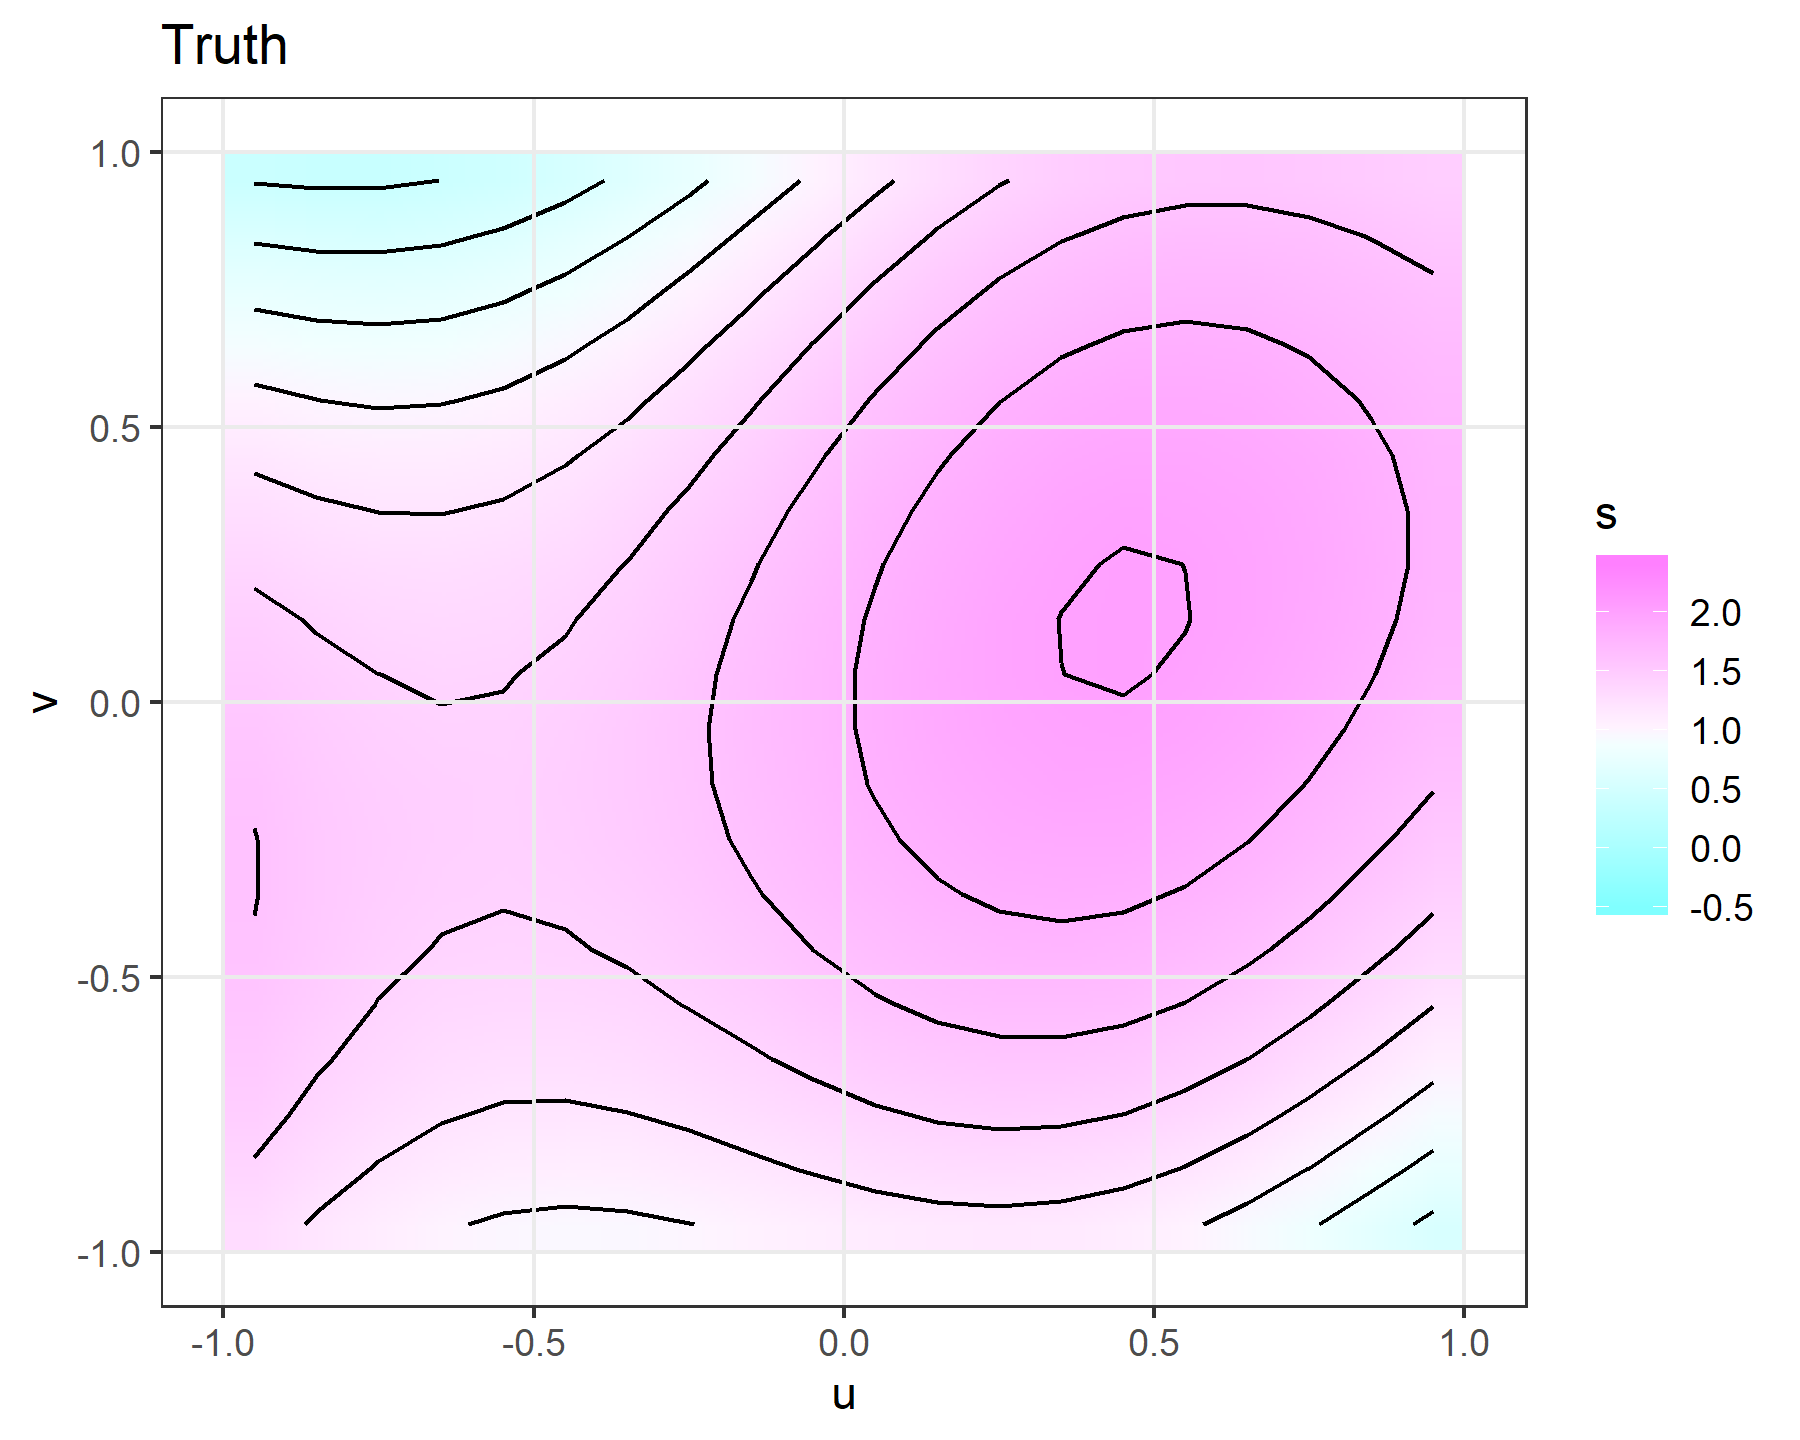
\includegraphics[width=0.4\linewidth]{Figures/Chap5/Paper3_true.png}
		\caption{Simulated spatial risk pattern.}
		\label{f:trueSpatial}
	\end{figure}
	
	\subsection{Spatial pattern recreation}
	In this section, we aimed to compare the performance of our proposed generalized additive mixed models in terms of spatial pattern recreation. Binary responses were then simulated via the model
	
	\begin{equation}\label{eq:simSP1}
	\mathbf{P}(y_{ij}=m) = p_{ij}^m(1-p_{ij})^{(1-m)},\ m=0,1
	\end{equation}
	where 
	\begin{equation}\label{eq:simSP2}
	\text{logit}(p_{ij}) = \beta_x x_{ij} + \beta_t t_{ij} + s_0(u_{ij},v_{ij}) + b_{0i} ,
	\end{equation}
	and $b_{0i} \stackrel{i.i.d.}{\sim} N(0,\tau_0^2)$. We repeated the simulation with $\tau_0=0,0.3,0.6,0.9$, respectively. 
	
	We sought to compare our proposed GAMM (given in (\ref{mod:gammsim})) with a naive GAM that assumes independent data (given in (\ref{mod:gamsim})):
	\begin{equation}\label{mod:gammsim}
	\text{logit}(p_{ij}) = \beta_0 +\beta_x x_{ij}+ \beta_t t_{ij} + lo(u_{ij},v_{ij}) + b_{0i} 
	\end{equation}
	\begin{equation}\label{mod:gamsim}
	\text{logit}(p_{ij}) = \beta_0 + \beta_x x_{ij}+ \beta_t t_{ij} + lo(u_{ij},v_{ij})
	\end{equation}
	
	We compared the estimated spatial risk patterns between the 2 models under varying random intercept conditions. Span sizes that minimize AIC \citep{akaike1998information} were chosen for classic GAM while our proposed OLMC method is used to choose span size for the GAMM. Note that if $\tau_0^2>0$, there will be individual-specific intercepts hence the model given in (\ref{mod:gamsim}) is a misspecified model due to its failure to account for the random effect. It follows that the likelihood of Model (\ref{mod:gamsim}) used in the AIC calculation would be incorrect hence the chosen span size tends not be the most appropriate, however a search across different span sizes did not return qualitatively different results from what is presented here. 
	
	The estimated spatial risk patterns are shown in Figure \ref{f:SpatialEsts3}. It is easily seen that that with correctly specified random effects, our proposed additive mixed models estimate the spatial patterns in a more precise fashion. In contrast, since the naive additive model fails to account for within-subject correlation, results for the model given in (\ref{mod:gamsim}) tend to under-smooth the patterns using a relatively small span sizes. This is due to the fact that the naive additive model treats correlated data as independent, resulting in an improper contribution of the correlated data to the total likelihood. 
	
	% f:SpatialEsts3 about here
	\begin{figure}[h]
		\centering
		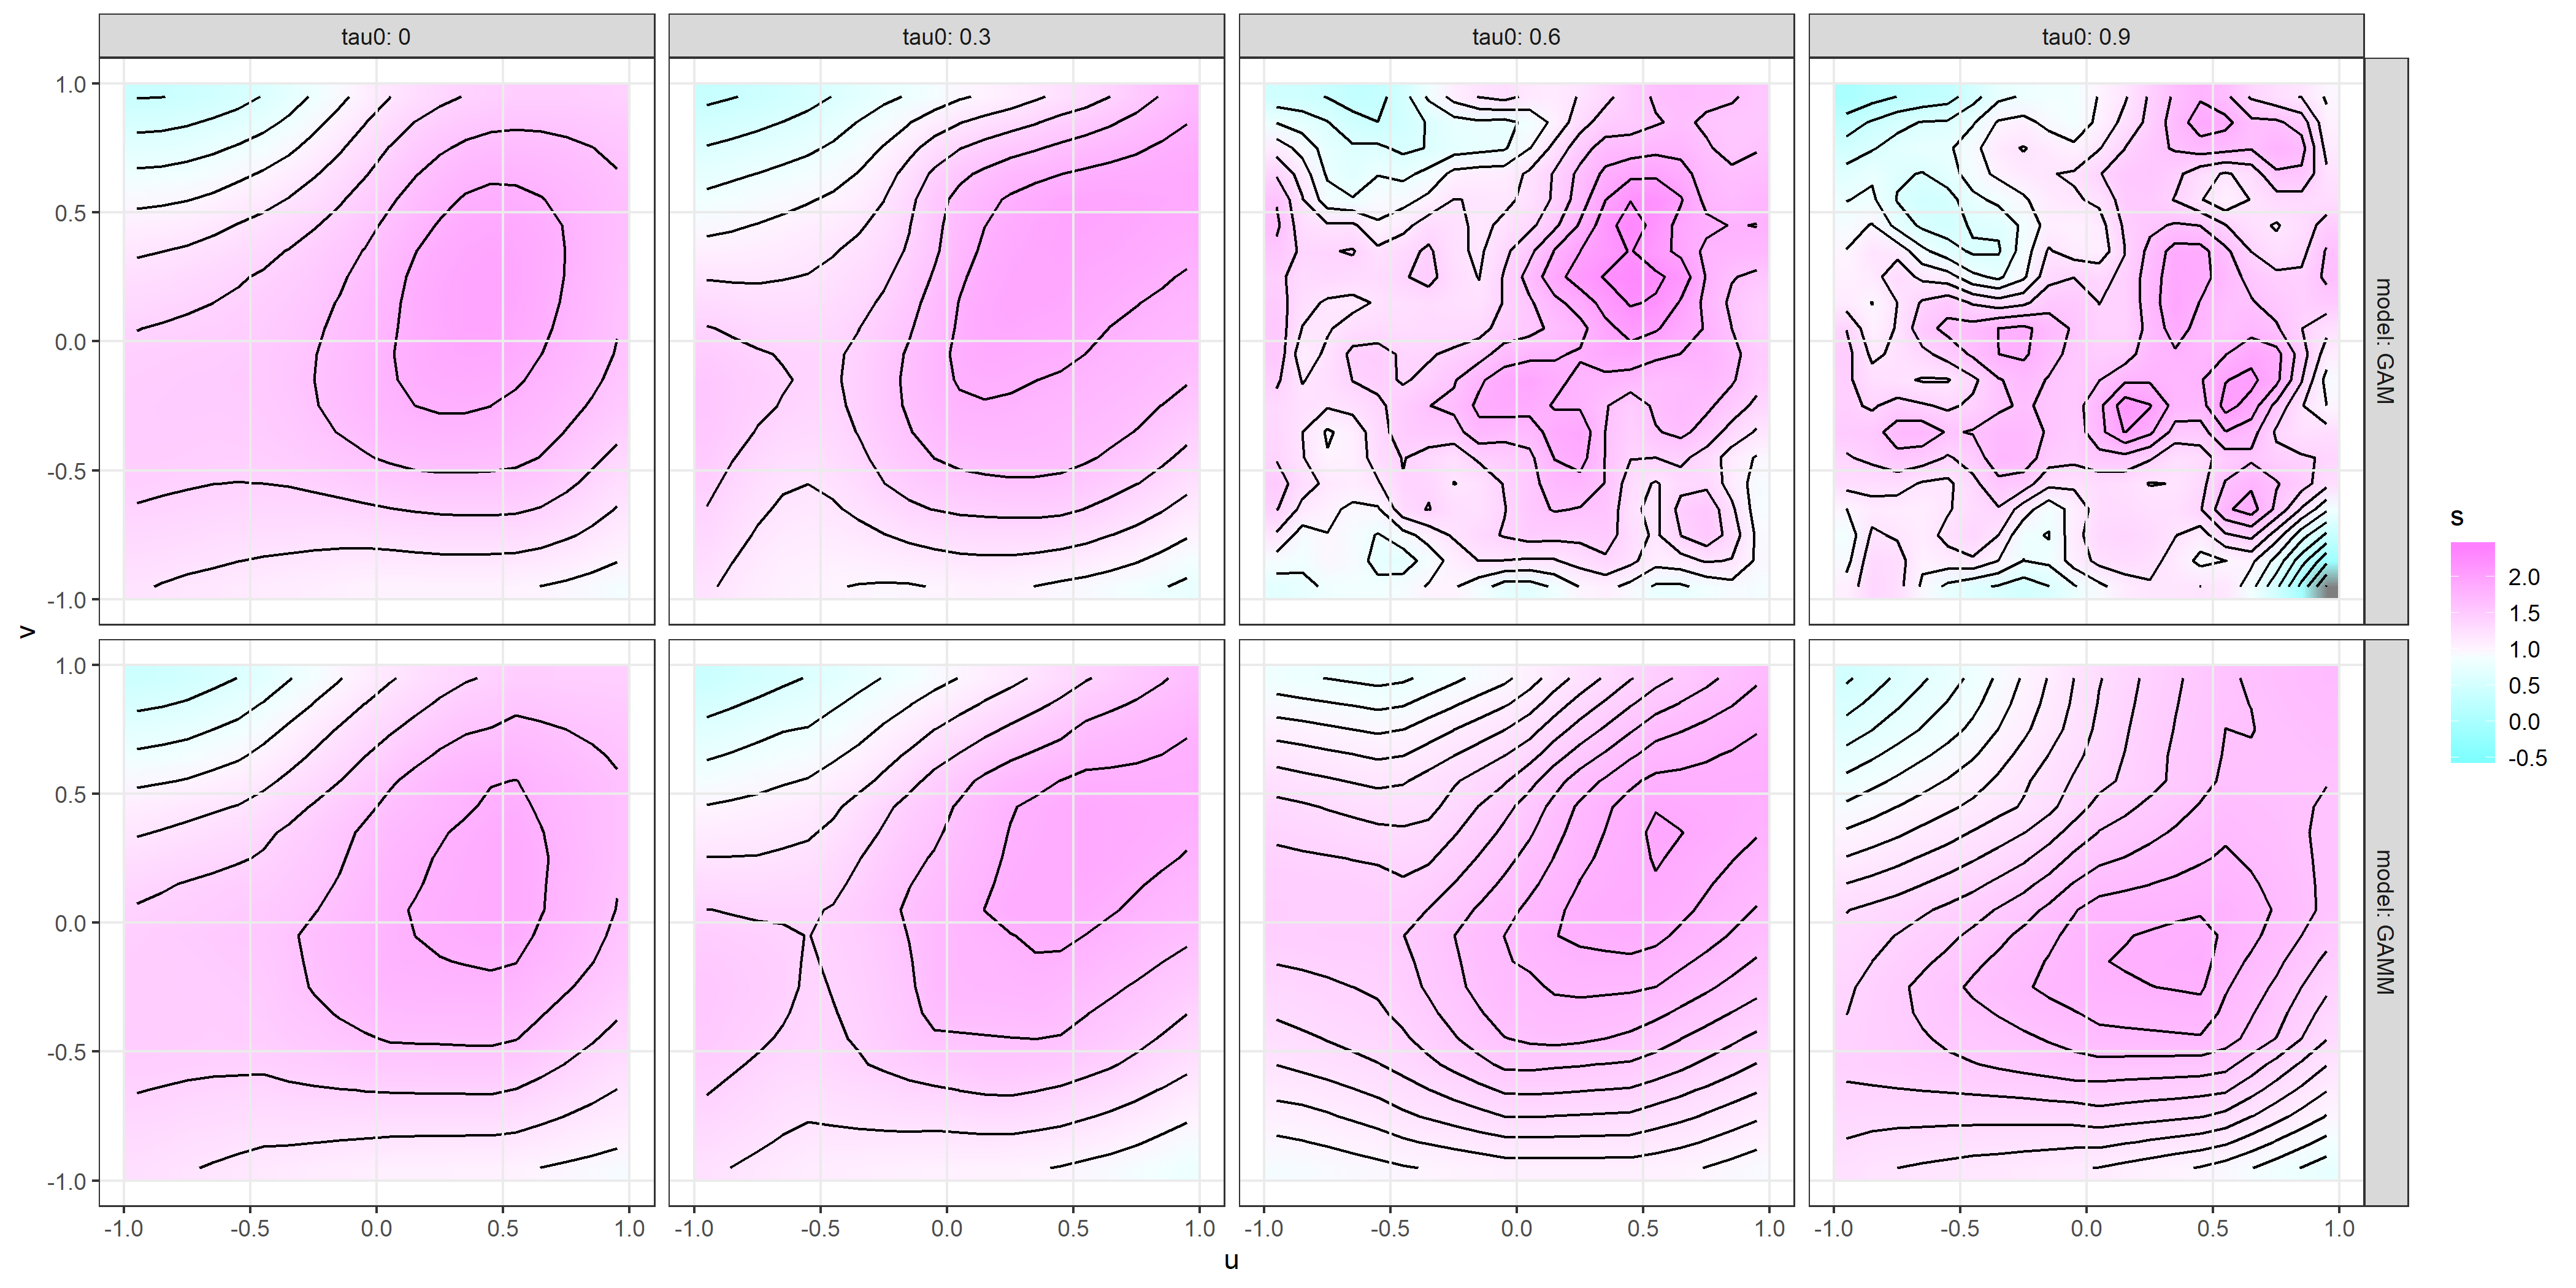
\includegraphics[width=1\linewidth]{Figures/Chap5/Comb_ests.png}
		\caption{Top: estimated patterns using GAMs given differing true correlation structures; Bottom : estimated patterns using GAMMs given differing true correlation structures.}
		\label{f:SpatialEsts3}
	\end{figure}
	
	\subsection{Quantification of uncertainty of estimated spatial effects}
	To access the performance of our proposed methods to quantify the uncertainty of estimated spatial effects discussed in \ref{s:fitting}, simulated data were created using (\ref{eq:simSP2}), where $b_{0i} \stackrel{i.i.d.}{\sim} N(0,\tau^2)$. 3 scenarios were designed with $\tau=0.2,\ 0.4,\ 0.6$, respectively. 300 repetitions were performed for each scenario. For each repetition, 95\% CIs are derived using our proposed method for every location on a uniformly designed $20\times 20$ grid on the map. Both sample mean and sample standard deviation of the coverage were reported in Table \ref{t:sim3coverage}. From the results, The uncertainty in spatial effects was well estimated and the 95\% confidence intervals managed to render the target coverage. 
	
	\begin{table}[h]
		\caption{Sample mean and sample standard deviation of the coverage proportion of 95\% confidence intervals of spatial effects. Coverage proportions are computed based on 300 repetitions while mean and standard deviation are calculated over 400 locations on map.
			\label{t:sim3coverage}}
		\centering
		\begin{tabular}{cccc}
			\hline
			$\tau_0$ & mean coverage & s.d. \\
			\hline
			0.2 &  0.939 & 0.039\\
			0.4 &  0.947 & 0.055\\
			0.6 &  0.979 & 0.030\\
			\hline
		\end{tabular}
	\end{table}
	
	\subsection{Parameter estimation}
	In this section, we investigated the performance of our proposed GAMMs in terms of point estimation of the parameters in both the fixed effects and the variance of random effects via a new set of simulation studies where responses were simulated using model 
	\begin{equation}\label{eq:simrand}
	\text{logit}(p_{ij}) = \beta_x x_{ij} + \beta_t t_{ij} + s_0(u_{ij},v_{ij}) + b_{0i} + b_{1i}t_{ij},
	\end{equation}
	with $b_{0i} \stackrel{i.i.d.}{\sim} N(0,\tau_{0}^2)$ and $b_{1i} \stackrel{i.i.d.}{\sim} N(0,\tau_{1}^2)$.
	
	On the simulated dataset, we sought to access the performance of our proposed GAMM given by 
	\begin{equation}\label{mod:ammsim2}
	y_{ij} = \beta_0 + \beta_x x_{ij} + \beta_t t_{ij} + lo(u_{ij},v_{ij}) + b_{0i} + b_{1i}t_{ij}.
	\end{equation}
	The estimated values of $\beta_x$, $\beta_t$, $\tau_{0}$ and $\tau_{1}$ were recorded. The corresponding results presented in Table \ref{t:parameterests} were based upon a total of 300 simulations. The sample mean and standard deviation of estimated model parameters, along with the mean estimated standard deviations, were reported. From the results, it could be seen that by correctly accounting for the correlation structure, our proposed GAMMs managed to both estimate parameters in fixed effects with less bias. On the other hand, GAMMs accounted for the individual-specific random effects and hence managed to estimate the variance of the random effects. 
	
	% t:parameterests about here
	% latex table generated in R 3.6.0 by xtable 1.8-4 package
	% Sat Jul 25 16:02:17 2020
	\begin{table}[h]
		\caption{Parameter estimation based on 300 repetitions
			\label{t:parameterests}}
		\centering
		\begin{tabular}{llrrlll}
			\hline
			model & parameter & truth & mean of estimates & relative bias & empirical s.d. & mean of $\hat{s.d.}$ \\     \hline
			GAM & $\beta_x$ & 0.20 & 0.17 & -17\% & 0.033 & 0.031 \\ 
			& $\beta_t$ & -0.10 & -0.09 & 12\% & 0.0034 & 0.0032 \\ 
			GAMM & $\beta_x$ & 0.20 & 0.19 & -5.5\% & 0.035 & 0.032 \\ 
			& $\beta_t$ & -0.10 & -0.10 & 4\% & 0.004 & 0.0041 \\ 
			& $\tau_0$ & 0.50 & 0.53 & 6.6\% & - & - \\ 
			& $\tau_1$ & 0.07 & 0.07 & -5.7\% & - & - \\ 
			\hline
		\end{tabular}
	\end{table}
	
	
	\section{Application to serum PFOA study}
	In this section, we apply our proposed GAMM to estimate the spatial risk pattern of high serum PFOA concentration with adjustment of relevant confounding covariates. Here we focus on a approximate square map defined within longitude $81^{\circ} 30'\  W$ - $81^{\circ} 50'\  W$ and latitude $39^{\circ} 07'\  N$ - $39^{\circ} 27'\  N$, which is approximately a $23\times 23$ square in miles around Lubeck, WV area. Within this area, 1070 records on 193 individuals are available where 140 of them have 6 measurements of serum PFOA concentration. Among the 193 residents, 99 are female and 94 are male. Age at baseline has mean 54.6 and standard deviation 14.9 with minimum 19 and maximum 92. We use 100 ng/mL as a threshold for ``high concentration" where serum PFOA concentration values that are greater than 100 ng/mL are considered high. 
	
	To estimate the spatial pattern of residents' high serum PFOA concentration risk with control of gender, age and a linear trend in time, we fitted an GAMM given by 
	
	\begin{equation}\label{mod:PFOA}
	g(p_{ij}) = \beta_0 + \beta_1 female_i + \beta_2 age_i + \beta_3 t_{ij} + lo(u_{ij}, v_{ij}) +  b_{0i}, 
	\end{equation}
	where $p_{ij}$ is the probability that individual $i$ has a high serum PFOA concentration at time $j$ and $b_{0i} \stackrel{i.i.d.}{\sim} N(0,\tau_0^2)$. 
	
	The fitted spatial pattern of log-odds, along with point-wise 95\% confidence intervals, is shown in Figure \ref{f:pfoaplotsGAMM}. From the results, it could be seen that potential high PFOA risk areas exist in western and north-eastern parts of the area. Further point-wise significance tests are performed at each location within a uniformly designed $20\times 20$ grid on the map of interest. Specifically, 95\% confidence interval of spatial effect at each location is compared with the mean estimated spatial effect over the 400 locations. A location is labeled as significant if the 95\% CI at the location does not cover the mean estimated effect. The results are plotted in Figure \ref{f:pfoasigs3}, from which significantly higher risks are observed at 129 locations while significantly lower risks are observed at 175 locations, indicating significant geospatial disparity in residents' serum PFOA concentration over the map. These results could potentially help epidemiologists on further space-confounded risk factor detection. 
	
	
	\begin{figure}[h]
		\begin{center}
			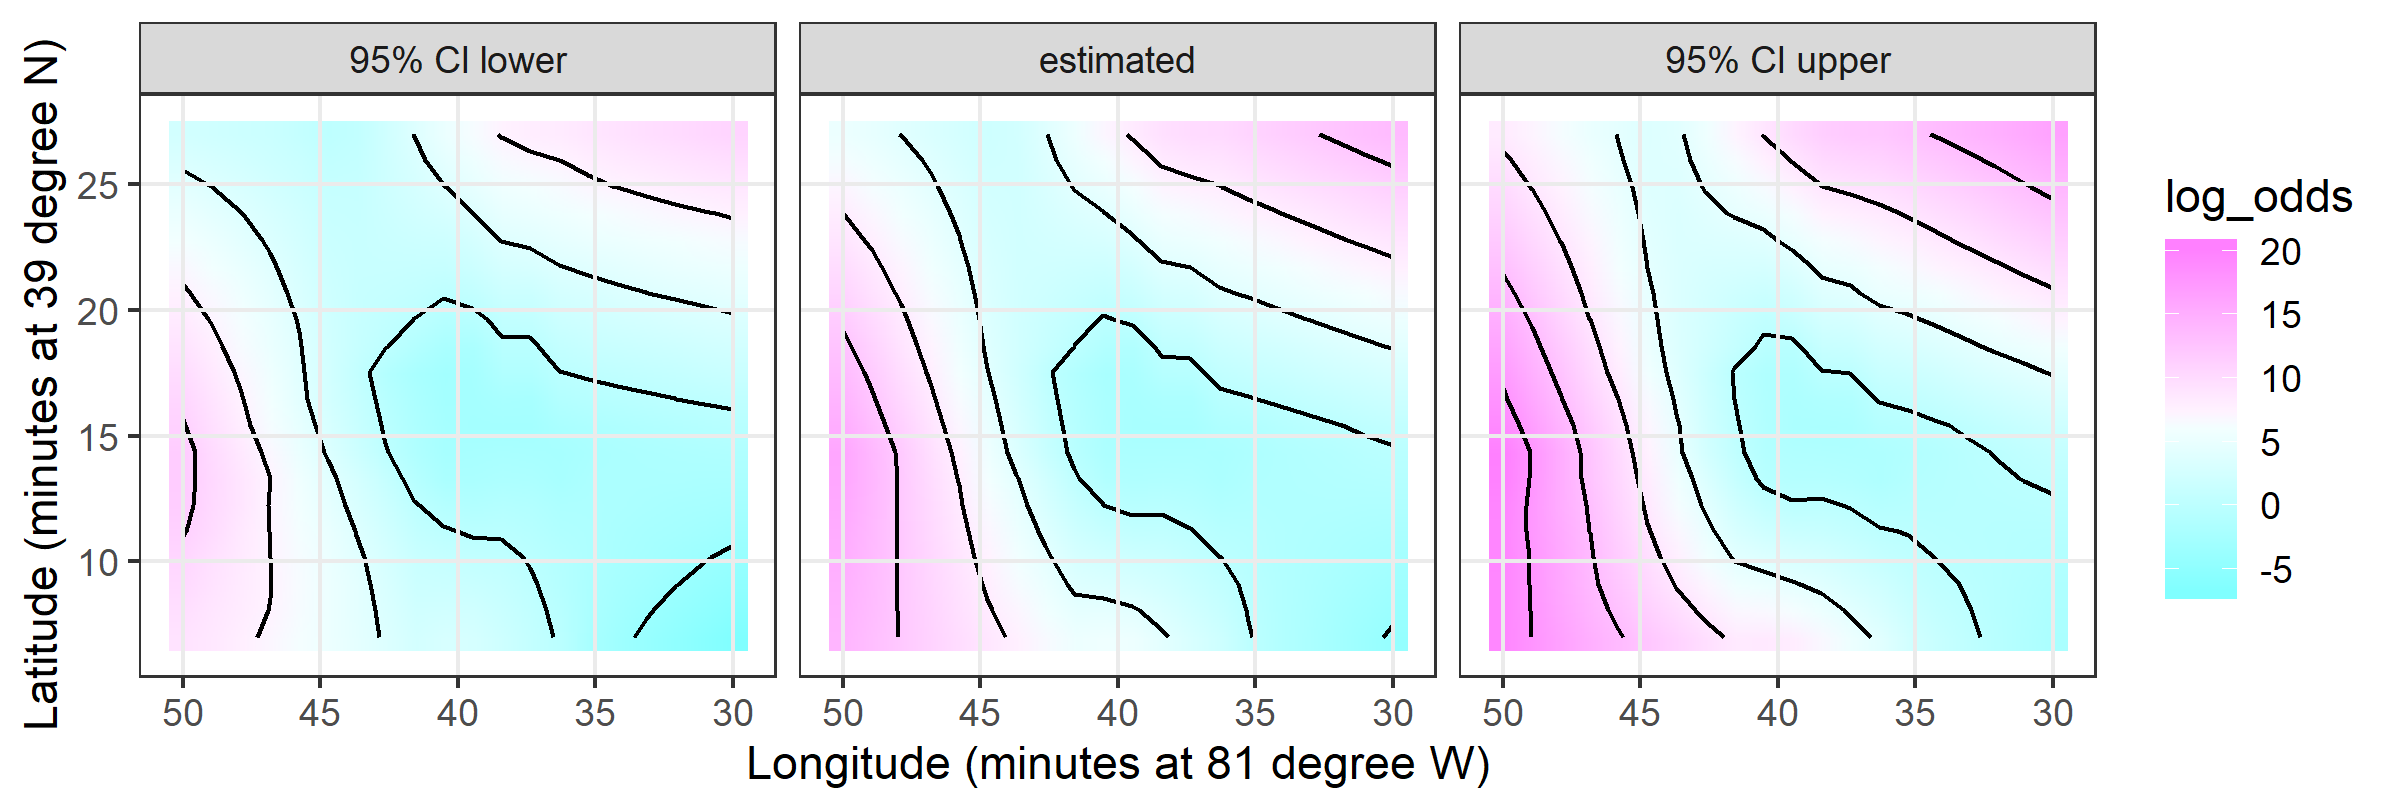
\includegraphics[width=\linewidth]{Figures/Chap5/Ests3.png}
		\end{center}
		\caption{Left: point-wise lower bounds of 95\% CIs ; Middle: estimated pattern of log odds ratio of high serum PFOA using Model (\ref{mod:PFOA}); Right: point-wise upper bounds of 95\% CIs.}
		\label{f:pfoaplotsGAMM}
	\end{figure}
	
	\begin{figure}[h]
		\begin{center}
			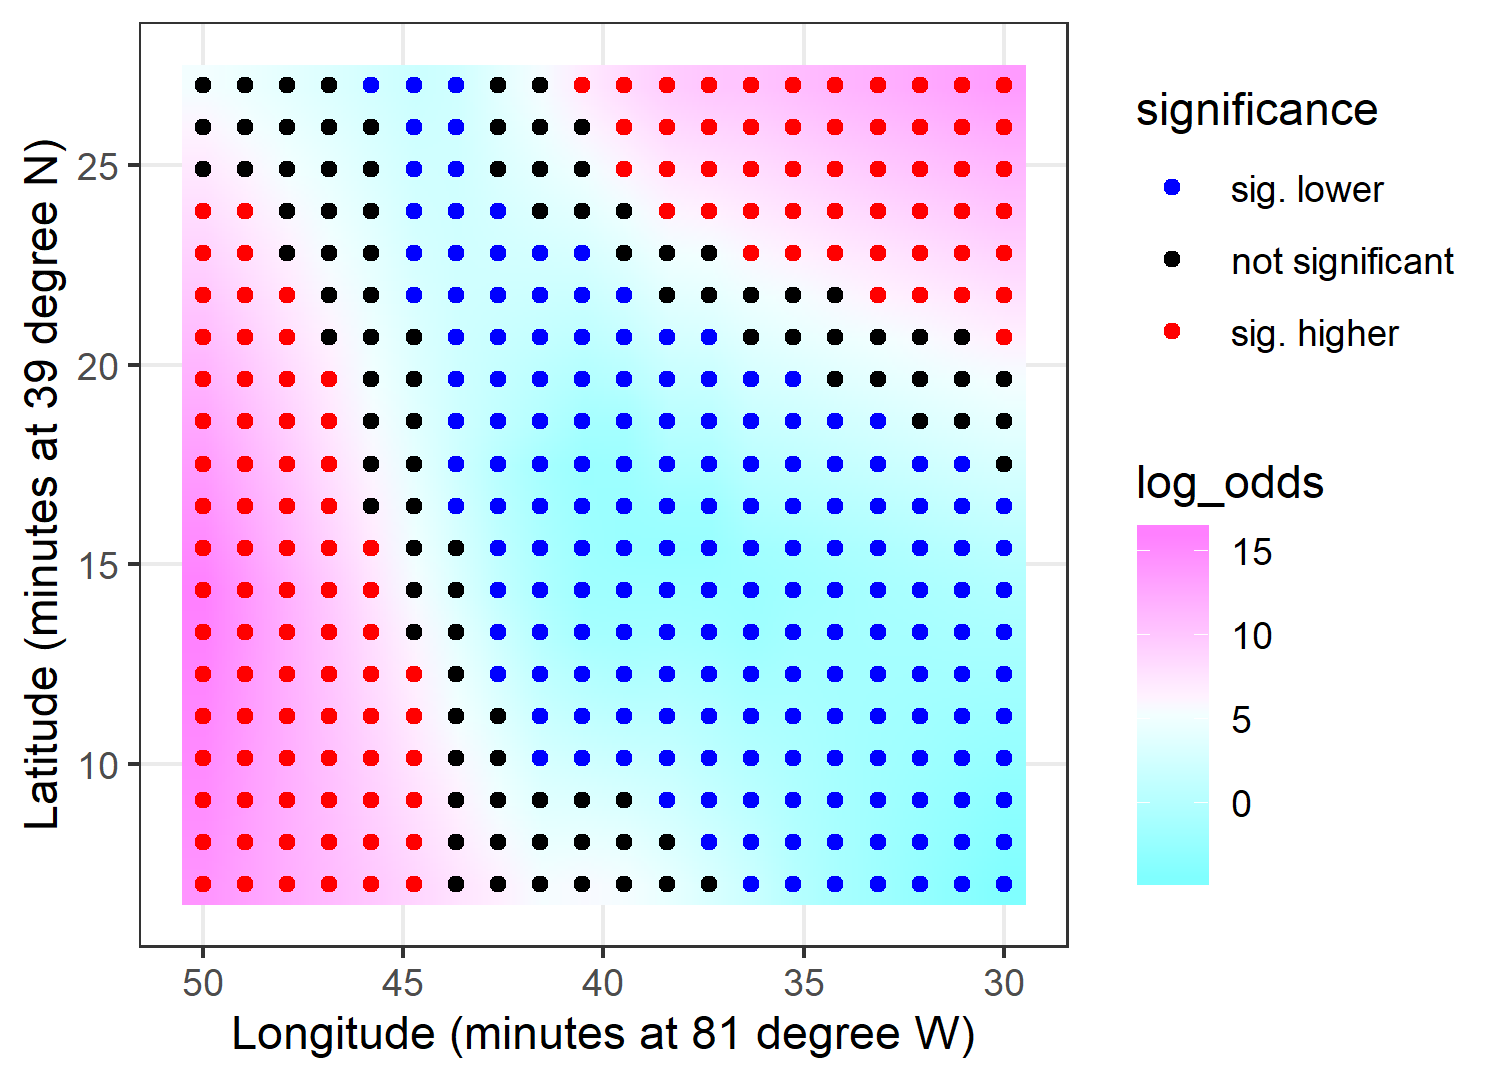
\includegraphics[width=0.5\linewidth]{Figures/Chap5/sig3.png}
		\end{center}
		\caption{Significance of the grid locations on the estimated spatial effects map.}
		\label{f:pfoasigs3}
	\end{figure}
	
	\section{Discussion}
	\label{s:discuss}
	We proposed a novel class of generalized additive mixed models that incorporate kernel smoothers. To achieve this, we combined PQL procedure and backfitting algorithm. To choose the proper amount of smoothing, we proposed an out-of-sample likelihood Monte Carlo method in order to avoid over-smoothing or under-smoothing. We showed that by adjusting for the correlation structure, our model better recreated the spatial risk pattern than a naively applied GAM. Empirical results also showed that our model managed to render estimation of parameters in both mean and variance components with less bias when the model was correctly specified. Our methods were further used in a recent study on residents' serum PFOA concentration in Lubeck, WV and spatial disparity in risk of high serum PFOA concentration was identified. 
	
	In this work, we focused on kernel smoothers, utilizing LOESS in particular in order to meet the demand of various spatial epidemiology studies. We mentioned but did not elaborate on the use of spline smoothers in the context, partially due to the fact that those models are relatively well investigated in existing literature such as \citet{wood2017generalized} and \citet{lin1999inference}. We did not cover Bayesian spatial estimation methods based on stochastic processes but we do recognize their popularity, as well.
	
	This work is a direct complement of the work of \citet{Tang2020Additive} by accommodating responses of exponential family. This work could also be viewed as the alternative to \citet{lin1999inference} when kernel smoothers are preferred over spline smoothers. This work was developed based on PQL procedure, which is one of the popular fitting procedure of a classic GLMM. One natural future direction is to develop a fitting procedure using marginal quasi-likelihood \citep{breslow1993approximate} for GAMM with kernel smoothers. 
	
	

%%% Local Variables: ***
%%% mode: latex ***
%%% TeX-master: "thesis.tex" ***
%%% End: ***
